\begin{figure}[htb]
	\begin{center}
		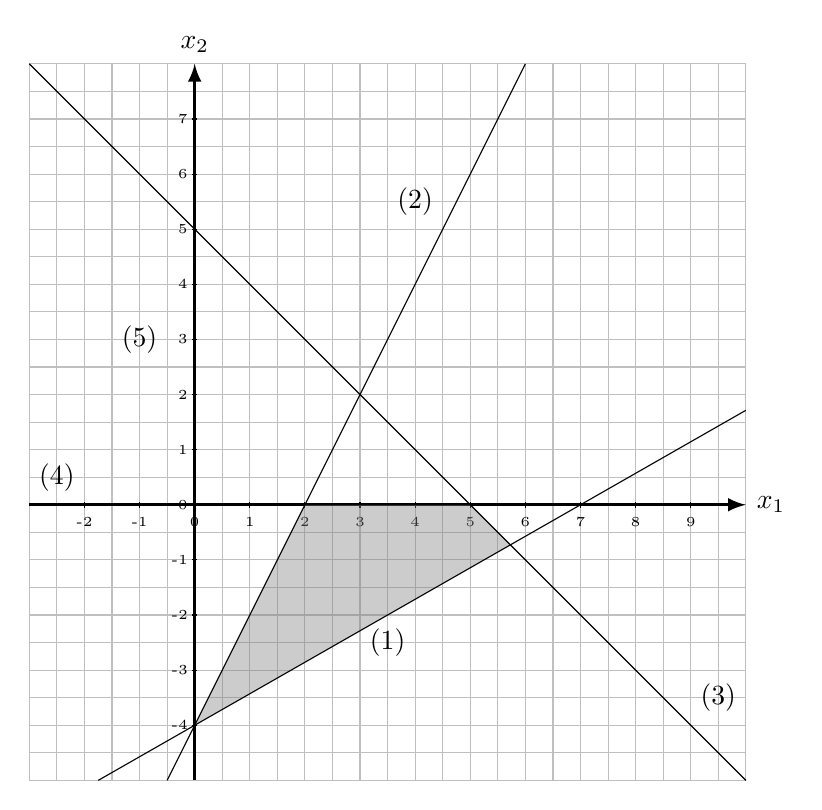
\begin{tikzpicture}[scale=0.7]
		\draw[gray!50, thin, step=0.5] (-3,-5) grid (10,8);
    	\draw[very thick,-latex] (-3,0) coordinate(x1) -- (10,0) coordinate(x2) node[right] {$x_1$};
    	\draw[very thick,-latex] (0,-5) coordinate(y1) -- (0,8) coordinate(y2) node[above] {$x_2$};
	    \foreach \x in {-2,...,9} \draw (\x,0.05) -- (\x,-0.05) node[below] {\tiny\x};
	    \foreach \y in {-4,...,7} \draw (-0.05,\y) -- (0.05,\y) node[left] {\tiny\y};
	
		\fill[gray,opacity=0.4] (0,-4) -- (63/11,-8/11) -- (5,0) -- (2,0)  --cycle; 
	
	    \draw (10,12/7)--(-7/4,-5);
	    \draw (-1/2,-5)--(6,8);
	    \draw (10,-5)--(-3,8);

		\node at (4, 5.5){(2)};
		\node at (3.5,-2.5){(1)};
		\node at (9.5, -3.5){(3)};
		\node at (-2.5,0.5){(4)};
	     \node at (-1,3){(5)};
		
	
		
		\end{tikzpicture}
		\caption{\label{fig:q19-feasible0}Feasible Domain}
	\end{center}
\end{figure}


Consider the optimization problem $\min 2 x_1 - x_2$, where ($x_1$, $x_2$) is constrained
to belong to the polyhedron  represented in Figure \ref{fig:q19-feasible0}.
\begin{enumerate}
\item Formulate the 5 constraints that determine the feasible domain represented in gray in Figure \ref{fig:q19-feasible0}. 


\item Write the corresponding linear optimization problem in standard form. 
Give explicitly the matrix $A$ and the vectors $b$ and $c$.


\item List the basic solutions of the problem. For each basic solution:
\begin{itemize}
\item   identify the solution on Figure \ref{fig:q19-feasible0},
\item  determine if the solution is feasible.
\end{itemize}

\item Is there any degenerate feasible solution? Justify. 

\item Why does point  $(2,$ $-2)$ represent a feasible solution, but not a basic solution?

\item  Consider the solution on Figure \ref{fig:q19-feasible0}  where constraints (2) and (5) are active,
 and the corresponding basic solution in the problem in standard form where the variables associated with these constraints are out of the basis.
 
\begin{enumerate}
\item Give the basis matrix.
\item Calculate all basic directions. Are the basic directions feasible? Justify your answer.\\
\end{enumerate}

\end{enumerate}


